\begin{frame}[fragile,c]{まとめ}
    \setlength{\leftmargini}{1em}

    \begin{figure}[H]
        \begin{minipage}[b]{0.55\hsize}
            \textbf{ポイント}
            \begin{itemize}
                \item 寿司は\alert{美味しい}
                \item おなかすいた
                \item Wikipediaは参考文献にならない
            \end{itemize}
             \\
            \textbf{今後の課題}
            \begin{itemize}
                \item 他都府県のお寿司はどうなのか
            \end{itemize}
        \end{minipage}
        \begin{minipage}[t]{0.4\hsize}
            \centering
            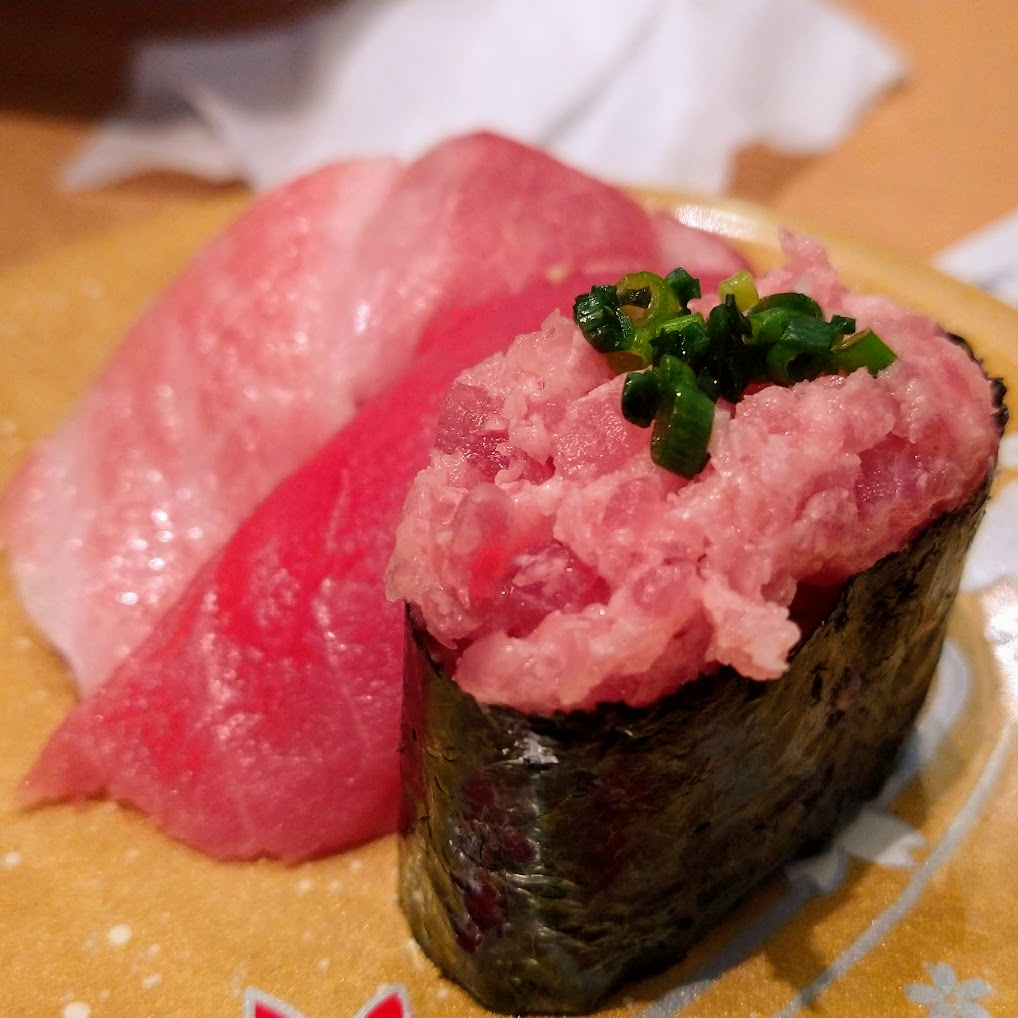
\includegraphics[width=0.95\hsize]{oishii}
            \caption{美味しい寿司}
            \label{fig:oishii}
        \end{minipage}
    \end{figure}

\end{frame}
